\chapter{Unity DOTS: Entity Component System}
\label{cap:ecs}
% NB: le parole al plurale in inglese vengono declinate al singolare in italiano, anche se la frase è al plurale

Per Unity, ECS è il nucleo della nuova tecnologia DOTS, in quanto è ciò che permette di realizzare il pattern data-oriented. Per utilizzarlo in un progetto dobbiamo importare il package \emph{Entities} (\verb|com.unity.entities|).

% esempio: come introdotto nella sezione ref... (citare)

%%%%%%%%%%%%%%%%%%%%%%%%%%%%%%%%%%%%%%%%%%%%%%%%%%%%%%%%%%%%%%%%%%%%%%%%%%%%%
\section{Introduzione a ECS}

Un'architettura di tipo ECS separa i tre concetti di entità, stato e comportamento, e si concentra sui dati di basso livello. I sistemi leggono stream di dati dei componenti, quindi li trasformano da dati di input a dati di output, e le entità indicizzano questi ultimi.

\paragraph{Archetipi}

Un \emph{EntityArchetype} è una combinazione unica di certi tipi di componenti. Ogni entità ne ha uno e quando vengono aggiunti o rimossi componenti all'entità, il suo archetipo cambia (esempio in Figura~\ref{fig:archetype}).

\begin{figure}[!ht]
    \centering
    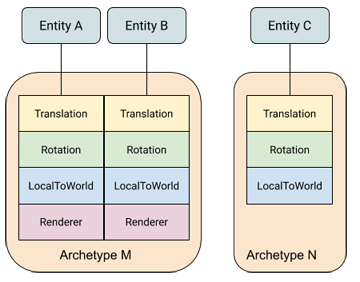
\includegraphics[width=0.60\columnwidth]{gfx/imgs/chapter2/ArchetypeDiagram.png}
    \caption{Esempi di archetipi: le entità A e B hanno lo stesso archetipo in quanto possiedono lo stesso set di componenti~\cite{doc:unity-entities-manual}.}
    \label{fig:archetype}
\end{figure}

\paragraph{Chunk di memoria}
L'archetipo di una entità determina dove i componenti di questa vengono memorizzati. ECS alloca memoria in blocchi chiamati \emph{ArchetypeChunk}, ognuno dei quali è rappresentato da un archetipo e contiene sempre e solo entità di quello stesso archetipo (Figura~\ref{fig:memory-chunk}). I chunk sono costituiti da array di componenti e, quando l'archetipo di un'entità cambia (ad esempio vengono aggiunti o rimossi componenti), questa viene spostata in un chunk differente.

\begin{figure}[!ht]
    \centering
    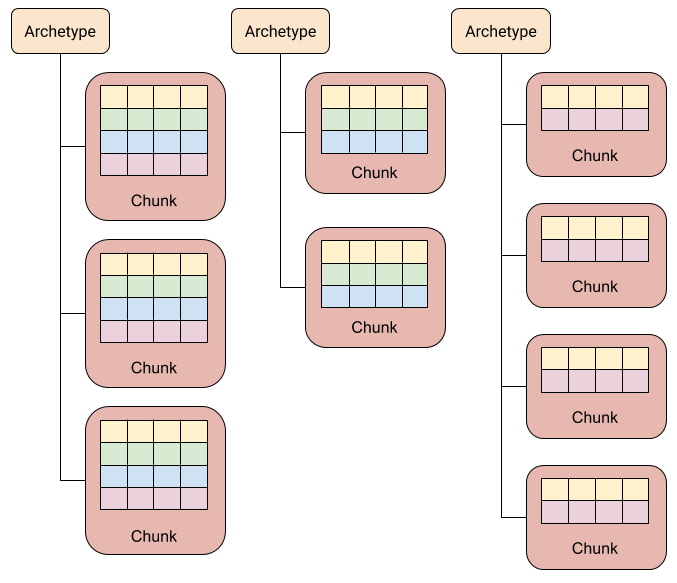
\includegraphics[width=0.85\columnwidth]{gfx/imgs/chapter2/ArchetypeChunkDiagramENG.png}
    \caption{Organizzazione delle entità nei chunk di memoria~\cite{doc:unity-entities-manual}.}
    \label{fig:memory-chunk}
\end{figure}

\paragraph{EntityQuery}

Quando realizziamo del comportamento, dobbiamo individuare quali entità il sistema deve processare. Per farlo utilizziamo, direttamente o indirettamente, una \emph{EntityQuery}. Questa non è altro che una descrizione delle entità su cui vogliamo iterare. Infatti, permette di cercare gli archetipi esistenti per le entità che hanno i componenti corrispondenti a quelli indicati, fornendo una lista dei chunk su cui possiamo iterare.

\paragraph{Jobs}

Il \emph{\Csh{} Job System} di Unity permette di sfruttare i vantaggi del multithreading per eseguire del comportamento in parallelo. A tal proposito ECS fornisce dei meccanismi (ad esempio, \verb|Entities.ForEach| di \verb|SystemBase|) che permettono di eseguire operazioni al di fuori del main thread. I job vengono schedulati in base alle dipendenze che hanno fra di loro e all'ordine in cui i sistemi sono organizzati.

Poiché ECS introduce tipi e costrutti nuovi, DOTS fornisce il package \emph{Jobs}, che estende le funzionalità del \Csh{} Job System di Unity con tipi utili e compatibili con le entità~\cite{doc:unity-jobs}.

\paragraph{Organizzazione dei sistemi}

I sistemi in ECS sono organizzati per \emph{world} e \emph{group}. Di base viene creato un mondo predefinito chiamato DefaultWorld, con un insieme prefissato di gruppi e sistemi. Quindi ECS trova tutti i sistemi (gli script del proprio progetto), li istanzia e li aggiunge al gruppo SimulationGroup nel DefaultWorld, se non specificato in modo differente. I sistemi vengono aggiornati, ovvero viene invocato il metodo \verb|OnUpdate()|, nell'ordine in cui sono posizionati all'interno del gruppo a cui appartengono, a meno che non lo specifichiamo manualmente.

\paragraph{Authoring data e runtime data}

Esistono due fondamentali tipi di dati in Unity: \emph{authoring data} e \emph{runtime data}. Gli authoring data sono tutti quei tipi ed oggetti che riguardano la creazione nell'editor, ad esempio i GameObject presenti nella scena. Questi sono ottimizzati per essere flessibili (facilmente leggibili e modificabili, infatti Unity fornisce il pannello \emph{Inspector} per accederli). Inoltre, negli authoring data esistono gerarchie, ogni oggetto ha un nome e ci sono diverse informazioni di cui non si ha veramente bisogno a runtime; i runtime data, invece, sono i dati a tempo di esecuzione in \emph{Play Mode}\footnote{Edit Mode e Play Mode sono le due modalità in cui possiamo eseguire Unity. In particolare, per entrare in play mode è possibile utilizzare l'apposito pulsante nell'editor, oppure lanciare un'applicazione standalone.}, ad esempio le entità ed i componenti. In particolare, i runtime data sono ottimizzati per le performance (efficienza delle cache, tempi di caricamento e streaming, dimensioni di distribuzione).

Unity DOTS dispone di un conversion workflow che ci permette di convertire i GameObject in entità, e questa conversione avviene nell'editor.

%%%%%%%%%%%%%%%%%%%%%%%%%%%%%%%%%%%%%%%%%%%%%%%%%%%%%%%%%%%%%%%%%%%%%%%%%%%%%
% Pagine API: ArchetypeChunk, Entity, EntityManager, IJobEntityBatch, EntityQuery, World, WorldFlags
\section{Entities}

Le entità rappresentano le ``cose'' individuali del nostro gioco/applicazione. Non contengono né dati né comportamento, piuttosto definiscono quali parti di dati dovrebbero stare insieme. Le entità sono essenzialmente il rimpiazzo dei GameObject ma, mentre questi ultimi non sono altro che dei contenitori, le entità rappresentano degli indici. Infatti, mentre i GameObject sono delle classi, le entità sono semplici strutture, che contengono solo un ID ed un numero di versione per verificare se l'ID è ancora valido. Per avere un più chiaro esempio, una entità è paragonabile alla chiave di una tupla di un database.

Il fatto che sia entità che componenti siano implementati tramite delle strutture è un aspetto molto significativo. Le strutture sono infatti il modo più efficiente di immagazzinare dati per CPU e memoria; e sono estremamente sicure dal punto di vista del multithreading e del typing~\cite{article:ecs-data-structures}.

Solitamente non utilizziamo mai direttamente l'ID o il numero di versione di una entità per accedervi, ma passiamo la struttura a dei metodi. A tal proposito esiste una struttura, chiamata \verb|EntityManager|, che gestisce tutte le entità di un world. Essa mantiene una lista delle entità ed organizza i dati associativi per ottenere performance migliori. L'\verb|EntityManager| contiene tutte le API per: creare, leggere, aggiornare e distruggere le entità. Ogni \verb|World| possiede un unico \verb|EntityManager|, il quale gestisce tutte le entità presenti nel mondo a cui esso è associato~\cite{doc:unity-entities-api}.

\subsection{Creazione delle entità}

Esistono diversi modi per creare le entità. Il più semplice ed utilizzato è quello che sfrutta il \emph{Conversion Workflow} di DOTS. Questo permette di convertire i GameObject ed i prefab presenti nell'editor in entità, semplicemente inserendoli all'interno di una subscene\footnote{Le SubScene di DOTS permettono di convertire in entità tutti i GameObject che contengono. Quando chiudiamo una subscene, viene scritta una copia binaria delle entità memorizzate in cache, che permette di velocizzare il caricamento della subscene a runtime. Così facendo l'applicazione diventa notevolmente scalabile.}. Un secondo metodo consiste nell'utilizzo dell'\verb|EntityManager|, che espone la funzione \verb|CreateEntity()| per:

\begin{itemize}
    \item Creare entità dato un array di \verb|ComponentType| o un \verb|EntityArchetype|.
    \item Copiare un'entità già esistente.
    \item Creare un'entità senza componenti. 
\end{itemize}

Le entità create in questo modo vengono aggiunte al \verb|World| in cui si trova l'\verb|EntityManager|~\cite{doc:unity-entities-api}.
   
\begin{figure}[!ht]
    \centering
    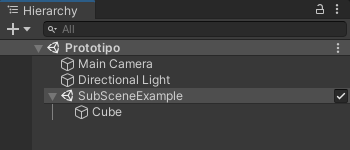
\includegraphics[width=0.70\columnwidth]{gfx/imgs/chapter2/SubSceneConversionWorkflow.png}
    \caption{Esempio di conversione di un GameObject ``Cube'' nella rispettiva entità, tramite subscene.}
    \label{fig:subscene-example}
\end{figure}

\subsubsection{Aggiunta e rimozione dei componenti}

Una volta creata una entità, possiamo aggiungervi o rimuoverne dei componenti utilizzando i metodi dell'\verb|EntityManager|. Quando ciò avviene l'archetipo dell'entità cambia ed ECS muove i dati in un nuovo chunk.

Le modifiche ad un'entità che causano cambiamenti strutturali (creazione$/$rimozione entità, aggiunta$/$rimozione di componenti e cambiamenti al valore di componenti condivisi) non sono operazioni thread-safe, quindi non possono essere effettuate all'interno di un job. Per eseguirle dobbiamo aggiungerle ad una struttura \verb|EntityCommandBuffer| ed applicarle una volta terminato il job~\cite{doc:unity-entities-api}.

\subsection{Accedere ai dati di un'entità}
In ECS, il modo più comune per accedere ai dati delle entità (ovvero al contenuto dei componenti) all'interno dei sistemi, è quello dell'iterazione. Tipicamente i sistemi ECS processano un set di entità, leggendo i dati da uno o più componenti, effettuando dei calcoli e scrivendo i risultati su altri componenti.
Il \Csh{} Job System permette di utilizzare i job per processare i componenti in parallelo, al fine di sfruttare al massimo la potenza di calcolo di tutti i core del processore e la località dei dati, evitando i cache misses.
ECS fornisce diverse API per realizzare l'iterazione, in particolare \verb|Entities.ForEach| all'interno di una classe \verb|SystemBase| (la classe per realizzare i sistemi), permette di utilizzare un \emph{lambda expression} per iterare su tutte le entità con un certo set di componenti.

La documentazione del package Entities sconsiglia di utilizzare alcuni costrutti, in quanto sono obsoleti e verranno deprecati in futuro~\cite{doc:unity-entities-manual}:
\begin{itemize}
    \item \verb|IJobChunk|.
    \item \verb|IJobForEach|.
    \item \verb|IJobForEachWithEntity|.
    \item \verb|ComponentSystem|.
    \item \verb|JobComponentSystem|.
\end{itemize}

\subsection{World}
Un \emph{world} organizza le entità, che esistono e hanno significato solo per il mondo in cui si trovano, in gruppi isolati. Esso possiede sia un \verb|EntityManager| che un set di sistemi, i quali possono accedere solo alle entità nel mondo di cui fanno parte.

Quando l'applicazione viene messa in esecuzione (o si entra in Play Mode) Unity crea un mondo di default chiamato DefaultWorld. Dopodiché istanzia tutti i sistemi (ovvero le classi che ereditano da \verb|ComponentSystemBase|, fra cui \verb|SystemBase|) e li aggiunge a tale mondo ~\cite{doc:unity-entities-manual}.

\paragraph{Gestione dei sistemi}
Uno dei compiti del mondo è quello di gestire i sistemi che vi fanno parte. Inoltre, la classe \verb|World| fornisce metodi per la creazione, l'accesso e la rimozione dei sistemi~\cite{doc:unity-entities-api}.

\paragraph{Tempo}
L'oggetto \verb|World| gestisce e controlla anche la proprietà \verb|Time| dei sistemi che vi fanno parte. Questa proprietà può essere utilizzata per ottenere il tempo nel mondo corrente e spesso è utile per definire comportamenti che utilizzano variabili dipendenti dal tempo (ad esempio la velocità).

\SaveVerb{TimeTerm}|Time|

\begin{lstlisting}[caption={Prototipo: utilizzo della proprietà \UseVerb{TimeTerm} per ruotare delle entità.},label={lst:time-property-example},language={[Sharp]C}]
public class RotateCollectibleSystem : SystemBase
{
    protected override void OnUpdate()
    {
        float deltaTime = Time.DeltaTime; // ottiene il tempo attuale

        Entities.ForEach((ref Rotation rotation, in RotationSpeedComponent rsc) =>
        {
            rotation.Value = math.mul(rotation.Value, quaternion.RotateX(math.radians(rsc.X * deltaTime)));
            rotation.Value = math.mul(rotation.Value, quaternion.RotateY(math.radians(rsc.Y * deltaTime)));
            rotation.Value = math.mul(rotation.Value, quaternion.RotateZ(math.radians(rsc.Z * deltaTime)));
        }).Run();
    }
}
\end{lstlisting}

Di default Unity crea una struttura \verb|TimeData| per ogni world. A tempo di esecuzione questa viene convertita in un'entità \verb|WorldTime|, che possiede un componente \verb|DeltaTime|. Quest'ultimo viene aggiornato continuamente dal sistema \verb|UpdateWorldTimeSystem| per rispecchiare il tempo passato rispetto al frame precedente. La proprietà \verb|Time| di un sistema è semplicemente un alias per l'entità \verb|WorldTime|.

\SaveVerb{WorldTimeTerm}|WorldTime|
\SaveVerb{DeltaTimeTerm}|DeltaTime|

\begin{figure}[!ht]
    \centering
    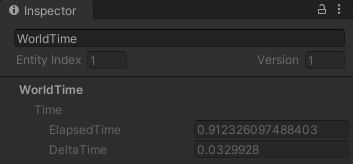
\includegraphics[width=0.65\columnwidth]{gfx/imgs/chapter2/WorldTimeEntity.png}
    \caption{Entità \UseVerb{WorldTimeTerm} ed il suo componente \UseVerb{DeltaTimeTerm} a runtime.}
    \label{fig:worldtime-entity}
\end{figure}

%%%%%%%%%%%%%%%%%%%%%%%%%%%%%%%%%%%%%%%%%%%%%%%%%%%%%%%%%%%%%%%%%%%%%%%%%%%%%
\section{Components}
I componenti rappresentano i dati del nostro gioco/applicazione, citando Maxim Zaks in ~\cite{article:components-definition}, essi sono «le parti atomiche dei nostri dati». In Unity ECS un componente è separato dal comportamento ed possiamo realizzarlo tramite una struttura che implementa una delle seguenti interfacce:
\begin{itemize}
    \item \verb|IComponentData|. È la più utilizzata e permette di definire un componente generico.
    \item \verb|IBufferElementData|. Permette di definire un componente contenente un buffer dinamico.
    \item \verb|ISharedComponentData|. Permette di definire un componente il cui valore viene condiviso da tutte le entità nello stesso chunk (ECS organizza o raggruppa le entità in base al valore di questo, all'interno di un archetipo);
    \item Componenti ibridi. Permettono di aggiungere i componenti di UnityEngine (GameObject) alle entità. Il principale motivo della loro esistenza è che DOTS è ancora in fase di sviluppo e molte feature di Unity ancora non hanno il corrispondente in ECS.
    \item \verb|ISystemStateComponentData|. Permettono di associare uno stato specifico di un sistema ad un'entità, rilevando quando le singole entità vengono create o distrutte.
    \item \verb|ISharedSystemStateComponentData|. Combina gli shared component ed i system state component.
    % RICONTROLLARE - blob footnote?
    \item \verb|BlobAsset|. Non è un vero e proprio componente ma possiamo utilizzarlo per memorizzare dati. Un blob (Binary Large OBject) asset è una struttura immutabile immagazzinata in memoria \emph{unmanaged} (ovvero per la quale non esiste un Garbage Collector che la pulisca), che può essere referenziato da uno o più componenti tramite \verb|BlobAssetReference|. Solitamente li usiamo per condividere dati fra asset e potervi accedere nei \Csh{} Job.
\end{itemize}

L'\verb|EntityManager| organizza combinazioni uniche di componenti tramite gli archetipi e memorizza i componenti di tutte le entità con lo stesso archetipo negli stessi chunk di memoria (tutte le entità in uno stesso chunk di memoria hanno tutte lo stesso archetipo)~\cite{doc:unity-entities-manual}.

I componenti di maggior interesse ai fini della tesi e dello sviluppo del prototipo sono \verb|IComponentData| e \verb|BufferElementData|. A tal proposito non tratteremo nel dettaglio gli altri, per i quali rimandiamo alla documentazione ufficiale~\cite{doc:unity-entities-manual}.

\subsection{Componenti generici}
Un componente generico è una struttura (quindi di default viene copiato per valore) che implementa l'interfaccia \verb|IComponentData|, fornita dal package Entities. Essendo una struttura, il componente può contenere solo tipi unmanaged e blittable, ovvero quei tipi di dato che vengono rappresentati nello stesso modo sia in memoria managed che unmanaged e non richiedono una gestione particolare da parte del marshaler di interoperabilità~\cite{doc:microsoft-blittable-types}.

Una singola implementazione di un componente dovrebbe contenere solo campi per dati che vengono acceduti sempre, o quasi, allo stesso tempo. Infatti, solitamente, avere un maggior numero di componenti piccoli è più efficiente rispetto all'avere pochi componenti ma grossi. Questo a causa del \emph{memory alignment} delle strutture: la CPU, per motivi di performance, memorizza i campi di una struttura sequenzialmente nell'ordine in cui sono dichiarati (il primo ha l'indirizzo di memoria più basso, l'ultimo il più alto). Ogni tipo di dato ha il proprio requisito di allineamento e, per le strutture, il requisito è il campo con la dimensione maggiore. Di conseguenza, se i campi sono di dimensioni diverse, solitamente la memoria totale allocata per la struttura è maggiore di quella minima che servirebbe, in quanto vengono inseriti degli offset per allineare i dati~\cite{doc:microsoft-memory-alignment}.

\verb|IComponentData| può anche essere implementato come classe, ad esempio per il porting in ECS di codice già esistente, ma ciò presenta numerosi svantaggi, ad esempio non può usufruire del Burst compiler (Sezione~\ref{subsubsec:impl-sistema}).

\begin{lstlisting}[caption={Prototipo: esempio di componente generico.},label={lst:generic-component-example},language={[Sharp]C}]
[GenerateAuthoringComponent]
public struct PlayerMovementSpeed : IComponentData
{
    public float speed;
}
\end{lstlisting}

\subsection{Aggiunta e rimozione dei componenti da un'entità}
L'\verb|EntityManager| espone metodi per aggiungere e rimuovere dei componenti da un'entità, e metodi per leggerne e impostarne il valore. Un'alternativa, è quella di utilizzare un \verb|EntityCommandBuffer|, una struttura thread-safe che permette di bufferizzare dei comandi (che agiscono anche su entità e componenti) per eseguirli più tardi, ma tutti in una volta nel frame.
Oltre a questi due metodi, ne esiste un terzo: aggiungendo l'attributo \verb|[GenerateAuthoringComponent]| alla struttura che implementa il componente, possiamo allegare il componente ad un GameObject presente nella scena. Così facendo, quando il GameObject verrà convertito in entità dal sistema di conversione, gli verrà assegnato tale componente.

\subsection{Accedere ai componenti di un'entità}
Solitamente l'accesso ai componenti viene fatto all'interno di un sistema, il quale itera su tutte le entità filtrate da una query che specifica un particolare set di componenti. Ad esempio, la query potrebbe specificare che devono essere filtrate solo le entità che hanno un componente \verb|PlayerMovementSpeed|, così che il sistema \verb|PlayerMovementSystem| possa implementare il movimento del giocatore e muovere solo l'entità del player.

\subsection{Buffer dinamici}
Un buffer dinamico è un particolare tipo di componente ECS che associa dei dati sotto forma di array ad una entità. È dinamico in quanto può contenere un numero variabile di elementi, ridimensionandosi automaticamente quando necessario. Possiamo anche specificarne una dimensione interna, tramite l'attributo \verb|[InternalBufferCapacity]|, che indica il numero di elementi che il buffer memorizza nell'ArchetypeChunk relativo. In tal caso, se il numero di elementi dovesse eccedere, il buffer allocherebbe un blocco di memoria heap (gestita completamente da ECS) fuori dal chunk, spostandovi tutti gli elementi~\cite{doc:unity-entities-manual}.

Per creare un buffer dinamico dobbiamo creare una struttura che implementa \verb|IBufferElementData|, definendo al suo interno il tipo di elemento che il buffer dovrà contenere.

\begin{lstlisting}[caption={Esempio buffer dinamico.},label={lst:dynamic-buffer},language={[Sharp]C}]
public struct IntBufferElement : IBufferElementData
{
    public int Value;
}
\end{lstlisting}

Per aggiungere il buffer ad un'entità, vi aggiungiamo semplicemente la struttura che implementa \verb|IBufferElementData|, come per un normale componente generico. \verb|EntityManager| e \verb|EntityCommandBuffer| espongono funzioni che permettono di aggiungere il buffer ad un'entità, restituendo una struttura container \verb|DynamicBuffer<T>|. Questa ci permette di accedere agli elementi \verb|inIBufferElementData| tramite un'interfaccia più ``array-like''.
Inoltre, \verb|DynamicBuffer<T>| fornisce un metodo \verb|Reinterpret<T>| che permette di reinterpretare il buffer con uno i cui elementi abbiano un tipo diverso, ma delle stesse dimensioni in memoria. Ciò permette di ottenere un handle sicuro per il buffer originale, utilizzando un riferimento, così che le modifiche siano correlate. Lo scopo è semplificare l'utilizzo del buffer, in quanto creare una struttura ogni volta per inserire un elemento può essere molto dispendioso e soggetto ad errori.

\SaveVerb{ReinterpretTerm}|Reinterpret<T>|

\begin{lstlisting}[caption={Esempio di utilizzo del metodo \UseVerb{ReinterpretTerm}.},label={lst:dynamic-buffer-reinterpret},language={[Sharp]C}]
DynamicBuffer<IntBufferElement> buffer1;
buffer.Add(new IntBufferElement() { value = 1 }); // dispendioso
DynamicBuffer<int> buffer2 = buffer1.Reinterpet<int>();
buffer2.Add(2); // semplice
\end{lstlisting}

%%%%%%%%%%%%%%%%%%%%%%%%%%%%%%%%%%%%%%%%%%%%%%%%%%%%%%%%%%%%%%%%%%%%%%%%%%%%%
\section{Systems}
Un sistema ECS è una classe che implementa il comportamento, fornendo la logica che trasforma i dati memorizzati in un componente dal suo stato corrente ad un altro stato. Un sistema opera su un insieme di entità che hanno un particolare set di componenti, specificato tramite una query, leggendo e scrivendo dati nei componenti di interesse.

\SaveVerb{DeleteTagComponentTerm}|DeleteTagComponent|
\SaveVerb{EntityCommandBufferTerm}|EntityCommandBuffer|

\begin{lstlisting}[caption={Prototipo: sistema che elimina tutte le entità che possiedono il componente \UseVerb{DeleteTagComponentTerm}, utilizzando un \UseVerb{EntityCommandBufferTerm}.},label={lst:system-simple-example},language={[Sharp]C}]
public class DeleteCollectibleSystem : SystemBase
{
    protected override void OnUpdate()
    {
        EntityCommandBuffer commandBuffer = new EntityCommandBuffer(Unity.Collections.Allocator.Temp);

        Entities
            .WithAll<DeleteTagComponent>()
            .ForEach((Entity entity) =>
            {
                commandBuffer.DestroyEntity(entity);
            }).Run();

        commandBuffer.Playback(EntityManager);
        commandBuffer.Dispose();
    }
}
\end{lstlisting}

% o subsub?
\paragraph{Cosa cambia rispetto ai MonoBehaviour classici}
Sia i sistemi che i MonoBehaviour sono classi e contengono metodi per realizzare il comportamento (i MonoBehaviour hanno la funzione \verb|Update()| che viene chiamata ad ogni frame, i sistemi hanno \verb|OnUpdate()|).

In Unity classico, quando vengono chiamate le \verb|Update()| di alcuni GameObject, anche se sono dello stesso tipo, tutte le operazioni vengono fatte sequenzialmente sul main thread. Quest'ultimo, infatti, itera su una lista di GameObject, accedendo al MonoBehaviour di ciascuno e chiamando per ciascuno la \verb|Update()| che realizza il comportamento. Ad esempio, se ci fossero dei GameObject zombie, significa che ognuno di questi muove se stesso per la mappa.
Al contrario, in ECS il sistema è completamente separato dalle entità su cui agisce: nel metodo \verb|OnUpdate()| vengono filtrate le entità con i componenti che vogliamo modificare, dopodiché vengono svolte delle operazioni su tali componenti. Quindi c'è un solo sistema che realizza una funzionalità specifica per tutte le entità coinvolte.

Così facendo si ottiene non solo separazione della logica, ma anche un modo semplice per realizzare le operazioni in parallelo, in quanto il codice dei sistemi può essere facilmente eseguito tramite job parallelizzabili. Inoltre, le operazioni di fetch delle entità su cui lavorare sono estremamente rapide, perché quelle con gli stessi componenti si trovano tutte raggruppate negli stessi chunk~\cite{youtube:differenze-unity-classico}.


\paragraph{Perché i sistemi sono così efficienti}
ECS è stato progettato avendo una chiara idea di come funziona l'hardware su cui il codice esegue.
Se il fetch della CPU avviene su dati che si trovano in cache di primo livello (le più efficienti), questa sarà un'operazione estremamente veloce, quindi sarebbe meglio sfruttarle il più possibile.

Nell'architettura classica, con i GameObject, ogni volta che la CPU caricava una cache line per mettere dei dati in cache, questa veniva riempita per buona parte di dati inutili. Ciò era dovuto al fatto che, anche se di un componente fosse servito solo il valore di un campo, la CPU lo avrebbe caricato comunque tutto nella cache line, compresi i dati superflui (un esempio è il componente Transform, che contiene moltissime dichiarazioni che raramente servono, vedi Figura~\ref{fig:transform-class}).

Al contrario, per com'è strutturato ECS, i componenti si trovano negli archetype chunk, dove i dati sono immagazzinati in array. Allineandosi perfettamente in memoria, possono essere caricati nella cache line con un overhead minimo.
Inoltre, ciò va anche a vantaggio del prefetching: non è difficile predire cosa succederà quando iteriamo su una serie di entità che hanno tutte gli stessi componenti, salvati in memoria in sequenze tutte uguali. Infatti, questo permette alla CPU di riconoscere il pattern e iniziare il fetching di due cache line alla volta. Ciò sarebbe stato impossibile con i GameObject, poiché spesso solo una piccolissima parte della cache line era utile alla CPU, mentre tutto il resto era da buttare~\cite{youtube:differenze-unity-classico}.

\subsection{Creazione di un sistema}
Per creare un sistema in Unity ECS è necessario implementare la classe astratta \verb|SystemBase| ed almeno il metodo di callback \verb|OnUpdate()|. Questo metodo viene chiamato ad ogni frame di esecuzione del gioco e viene attivato dalla \verb|OnUpdate()| del gruppo padre a cui il sistema appartiene.
Tutti gli eventi di un sistema eseguono sul main thread e solitamente all'interno di \verb|OnUpdate()| scheduliamo un job che esegue la maggior parte delle operazioni. Esistono diversi modi per farlo, in particolare:
\begin{itemize}
    \item \verb|Entities.ForEach|. È il modo più semplice ed utilizzato per iterare su componenti ECS.
    \item \verb|Job.WithCode|. Fornisce un meccanismo per implementare dei job singoli che possono eseguire anche in background, tramite una lambda expression.
    \item \verb|IJobEntityBatch|. fornisce un meccanismo di basso livello iterare su un set di istanze di \verb|ArchetypeChunk|, dove ogni istanza rappresenta un gruppo di entità in un chunk.
    \item \Csh{} Job System. permette di creare e schedulare job \Csh{} generici.
\end{itemize}

\subsubsection{Ciclo di vita di un sistema}
La classe \verb|SystemBase| da cui il sistema eredita, a seconda delle esigenze, può implementare le seguenti callback, che vengono chiamate in diversi momenti dell'esecuzione:
\begin{enumerate}
    \item \verb|OnCreate()|. Quando il sistema viene creato.
    \item \verb|OnStartRunning()|. Prima della prima \verb|OnUpdate()| ed ogni volta che il sistema riprende l'esecuzione.
    \item \verb|OnUpdate()|. Ad ogni frame fintanto che il sistema ha del lavoro da svolgere e la proprietà \verb|Enabled| è vera.
    \item \verb|OnStopRunning()|. Ogni volta che il sistema smette di aggiornare, ad esempio perché \verb|Enabled| è falso, oppure quando la query non trova entità corrispondenti al filtro. Viene anche chiamata prima di \verb|OnDestroy()|.
    \item \verb|OnDestroy()|. Quando il sistema viene distrutto.
\end{enumerate}

A meno che non scheduliamo dei job all'interno di \verb|OnUpdate()|, queste funzioni eseguono tutte sul main thread, nell'ordine mostrato in Figura~\ref{fig:system-callbacks}~\cite{doc:unity-entities-api}.

\SaveVerb{SystemBaseTerm}|SystemBase|

\begin{figure}[!ht]
    \centering
    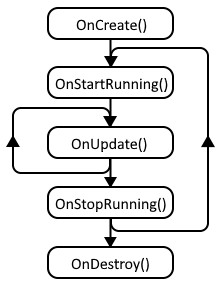
\includegraphics[width=0.34\columnwidth]{gfx/imgs/chapter2/SystemEventCallbacks.png}
    \caption{Callback di \UseVerb{SystemBaseTerm} e ordine in cui vengono chiamate.}
    \label{fig:system-callbacks}
\end{figure}

\subsubsection{Implementazione del comportamento con Entities.ForEach}
\label{subsubsec:impl-sistema}
La classe \verb|SystemBase| fornisce il costrutto \verb|Entities.ForEach| che permette di implementare ed eseguire gli algoritmi sulle entità in modo conciso. \verb|Entities.ForEach| esegue la funzione lambda su tutte le entità selezionate da una entity query: una volta definite le operazioni da eseguire all'interno della lambda expression, possiamo eseguire il job corrispondente con \verb|Run()| oppure schedularlo con \verb|Schedule()| o \verb|ScheduleParallel()|. 

\paragraph{Definizione della lambda expression}
Nella definizione della lambda expression dichiariamo dichiarati i parametri che il sistema utilizza per passare informazioni riguardanti l'entità corrente, quando la esegue.
Di default possiamo passare fino a otto parametri e devono essere raggruppati nell'ordine seguente: prima i parametri passati per valore \emph{senza keyword}, poi i parametri scrivibili passati per riferimento \emph{keywork `ref'}, infine i parametri di sola lettura passati per riferimento \emph{keyword `in'}. Per motivi di efficienza del job, è sempre meglio dichiarare con la keyword 'in' tutti i componenti di sola lettura~\cite{doc:unity-entities-api}.

Per accedere ad un componente associato ad un'entità, dobbiamo passare alla funzione lambda un parametro che ha come tipo il tipo del componente. Il compilatore aggiunge automaticamente i parametri nella definizione della query come componenti necessari.
Per i buffer dinamici la documentazione consiglia di utilizzare \verb|DynamicBuffer<T>| piuttosto che il tipo del componente (nell'esempio seguente è stato utilizzato per l'input del giocatore).
Esistono alcuni componenti speciali il cui valore è assegnato in base all'entità che il job della lambda sta attualmente processando, ad esempio Entity entity che corrisponde all'istanza dell'entità corrente.

\SaveVerb{PlayerMovementSystemTerm}|PlayerMovementSystem|

\begin{lstlisting}[caption={Prototipo: lambda expression di \UseVerb{PlayerMovementSystemTerm}, il quale aggiorna la velocità di un Player in base all'input.},label={lst:system-complex-example},language={[Sharp]C}]
#region Applicazione input

Entities.ForEach((DynamicBuffer<PlayerInput> inputBuffer, ref PhysicsVelocity pv,     in PredictedGhostComponent prediction, in PlayerMovementSpeed pms) =>
{
    if (!GhostPredictionSystemGroup.ShouldPredict(tick, prediction))
        return;
    
    PlayerInput input;
    inputBuffer.GetDataAtTick(tick, out input);
    var speed = pms.speed;
    if (input.horizontal > 0) 
        pv.Linear.x += speed * deltaTime;
    if (input.horizontal < 0) 
        pv.Linear.x -= speed * deltaTime;
    if (input.vertical > 0) 
        pv.Linear.z += speed * deltaTime;
    if (input.vertical < 0) 
        pv.Linear.z -= speed * deltaTime;
}).ScheduleParallel();

#endregion
\end{lstlisting}

\paragraph{Burst compiler}
\emph{Burst} (com.unity.burst) è uno dei package introdotti da Unity con DOTS. È progettato per lavorare con il Job System di Unity e permette di compilare il bytecode di .NET in codice nativo estremamente performante, semplicemente aggiungendo l'attributo \verb|[BurstCompile]| alla struttura del job~\cite{doc:unity-burst}.

Poiché nella \verb|OnUpdate()| di un sistema possiamo eseguire il job della lambda expression in modi diversi (\verb|Run()|, \verb|Schedule()|, \verb|ScheduleParallel()|), in base a questi vi sono dei vincoli differenti su come i dati vengono acceduti. Per questo motivo, molte delle funzionalità offerte da \verb|Entities.ForEach|, nel caso il job venga eseguito sul main thread con \verb|Run()|, entrano in conflitto con Burst, che non può essere utilizzato. In questo caso dobbiamo specificare ad ECS che non si vuole utilizzare Burst per il job di \verb|Entities.ForEach|, aggiungendovi il metodo \verb|WithoutBurst()|~\cite{doc:unity-entities-manual}.


\subsection{Istanziare un sistema}
Unity trova automaticamente le classi dei sistemi nel nostro progetto e le istanzia a runtime. Se non specificato in modo differente, di default i sistemi vengono aggiunti ad uno dei gruppi predefiniti (solitamente \verb|SimulationSystemGroup|), nel default world.

L'aggiornamento di un sistema, ovvero la chiamata del suo metodo \verb|OnUpdate()|, è gestita dal gruppo padre, a cui il sistema appartiene. Infatti, un gruppo non è altro che un tipo di sistema speciale che si occupa dell'aggiornamento dei figli.
ECS fornisce uno strumento, chiamato \emph{EntityDebugger} (vedi Figura~\ref{fig:entity-debugger}), per analizzare le entità e le gerarchie di sistemi presenti nei vari world dell'applicazione, sia in Edit Mode che in Play Mode.

\begin{figure}[!ht]
    \centering
    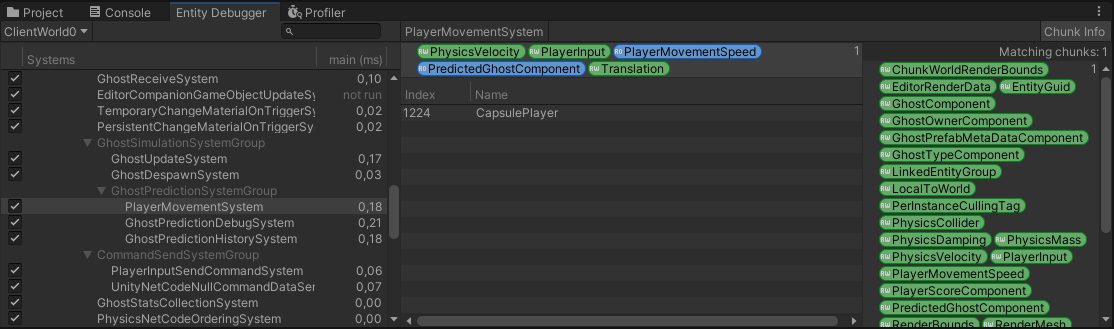
\includegraphics[width=0.95\columnwidth]{gfx/imgs/chapter2/EntityDebugger.png}
    \caption{Entity Debugger in Play Mode che mostra i sistemi in esecuzione in ClientWorld0.}
    \label{fig:entity-debugger}
\end{figure}

\subsection{Ordine di aggiornamento dei sistemi}
Generalmente i sistemi vengono aggiornati nell'ordine in cui sono inseriti nel gruppo padre. Per modificare manualmente l'ordine, possiamo utilizzare gli attributi \verb|[UpdateBefore]| e \verb|[UpdateAfter]| che indicano rispettivamente prima e dopo quale gruppo il sistema dev'essere aggiornato. Inoltre, possiamo specificare il gruppo padre con l'attributo \verb|[UpdateInGroup]|.
ECS di default crea una gerarchia di gruppi e sistemi che si dirama da tre nodi principali per tre particolari fasi del player loop (il ciclo di esecuzione della Play Mode):
\begin{itemize}
    \item \verb|InitializationSystemGroup|. Aggiornato alla fine della fase Initialization del player loop.
    \item \verb|SimulationSystemGroup|. Aggiornato alla fine della fase Update del player loop.
    \item \verb|PresentationSystemGroup|. Aggiornato alla fine della fase PreLateUpdatee del player loop.
\end{itemize}

Questa gerarchia non è statica, sia perché possiamo modificarla aggiungendo gruppi e sistemi, sia perché con certi package Unity aggiunge ulteriori gruppi. Ad esempio, utilizzando NetCode, vengono aggiunti i gruppi \verb|ClientSimulationSystemGroup| e \verb|ServerSimulationSystemGroup| che si occupano di aggiornare la simulazione rispettivamente solo sui client e solo sul server~\cite{article:player-loop-groups, doc:unity-entities-manual}.

\subsubsection{Entity Command Buffer}
Gli \verb|EntityCommandBuffer| sono strutture che permettono di accodare dei comandi eseguiti sul main thread o un job, così che possano essere eseguiti più avanti sul main thread e tutti insieme nello stesso frame.
Lo scopo di questa classe è risolvere due principali problemi: 
\begin{enumerate}
    \item All'interno di un job non è possibile accedere all'\verb|EntityManager| (quindi nemmeno all'interno di \verb|Entities.ForEach|).
    \item Quando viene eseguita un'operazione che causa un \emph{cambiamento strutturale} si genera un \emph{punto di sincronizzazione}.
\end{enumerate}

Il modo più efficiente di usare gli \verb|EntityCommandBuffer| è sfruttare uno dei tanti sistemi che li gestiscono, ad esempio \verb|EntityCommandBufferSystem|. Questi forniscono delle istanze di oggetti \verb|EntityCommandBuffer|, utilizzabili anche all'interno di altri sistemi, i cui comandi verranno eseguiti in sequenza nell'ordine in cui vengono inseriti. Nel caso ci servisse più di un buffer, i sistemi EntityCommandBufferSystem li gestiscono eseguendoli nell'ordine in cui sono stati creati.
Questo ci permette di creare un singolo punto di sincronizzazione quando \verb|EntityCommandBufferSystem| viene aggiornato, piuttosto che uno per ogni \verb|EntityCommandBuffer|, e garantisce determinismo.\\
Nel caso il job esegua in parallelo (ad esempio tramite \verb|ScheduleParallel()|), dobbiamo convertire l'\verb|EntityCommandBuffer| in uno concorrente, utilizzando il metodo \verb|AsParallelWriter()|~\cite{doc:unity-entities-api}.

\SaveVerb{EntityCommandBufferTerm}|EntityCommandBuffer|
\SaveVerb{OnUpdate()Term}|OnUpdate()|

\begin{lstlisting}[caption={Esempi di utilizzo di \UseVerb{EntityCommandBufferTerm}.}, label={lst:entitycommandbuffer-example}, language={[Sharp]C}]
var commandBuffer;

// esempio di creazione manuale di un command buffer
commandBuffer = new EntityCommandBuffer(Allocator.Temp);

// esempi di ottenimento di un command buffer da un sistema che li gestisce
commandBuffer = World.GetOrCreateSystem<EntityCommandBufferSystem>();
commandBuffer = World.GetOrCreateSystem<EndSimulationEntityCommandBufferSystem>();
commandBuffer = 
    World.GetOrCreateSystem<BeginInitializationEntityCommandBufferSystem>();

// creazione di un'entita' vuota e aggiunta di componenti
Entity ent = commandBuffer.CreateEntity();
commandBuffer.SetComponent(ent, new PlayerMovementSpeed() { speed = 10.0 });

// le operazioni seguenti non sono necessarie nel caso abbiamo ottenuto il buffer
// tramite uno dei sistemi descritti in precedenza.

// esegue in ordine tutte le operazioni accumulate nel buffer e ne libera la memoria
commandBuffer.PlayBack(EntityManager);
commandBuffer.Dispose();
\end{lstlisting}

\subsubsection{Punti di sincronizzazione}
Un punto di sincronizzazione è un momento nell'esecuzione del programma in cui aspettiamo il termine di tutti i job che sono stati schedulati prima. Essi impediscono di utilizzare tutti i worker thread disponibili nel job system per un certo periodo di tempo, perciò è meglio evitarli.
I punti di sincronizzazione sono causati principalmente dai cambiamenti strutturali, ovvero quelle operazioni che modificano l'archetipo di un'entità o cambiano l'ordine delle entità in un chunk. Esempi di cambiamenti strutturali sono la creazione e l'eliminazione di entità, l'aggiunta e la rimozione di componenti da un'entità e il cambiamento del valore dei componenti condivisi~\cite{doc:unity-entities-manual}. Per evitare i punti di sincronizzazione è possibile eseguire le operazioni che causano cambiamenti strutturali tutte insieme, tramite un \verb|EntityCommandBuffer|.

%\subsubsection{Job generici} % utile per prototipo? RICONTROLLARE
% Non serve perché li uso solo nei prototipi per gli stress test ma solo per creare le entities, non per mostrare il carico del lavoro. Per questo basta la parte sui system che fa ECS in background (.Run(), .Schedule() e .ScheduleParallel() sulla lambda)


%%%%%%%%%%%%%%%%%%%%%%%%%%%%%%%%%%%%%%%%%%%%%%%%%%%%%%%%%%%%%%%%%%%%%%%%%%%%%
\section{Conversion Workflow}
Unity ECS fornisce un meccanismo di conversione che permette di trasformare i GameObject (ed i MonoBehaviour associati), presenti in una scena, in entità. La differenza principale quando usiamo DOTS invece dell'architettura classica di Unity, è che invece di implementare dati e logica nei MonoBehaviour, definiamo i componenti per memorizzare dati a runtime e scriviamo i sistemi per realizzare la logica.

Per convertire un GameObject esistono due soluzioni: possiamo aggiungervi il componente \verb|ConvertToEntity| (MonoBehaviour), oppure inserirlo in una subscene. In entrambi i casi i sistemi di conversione forniti da DOTS processano il GameObject o il Prefab e tutti gli oggetti figli e li converte.
Tuttavia, la seconda soluzione è da preferire, in quanto con la subscene ECS serializza e salva su disco i dati delle entità che genera durante la conversione. Tali dati possono essere caricati o trasmessi in stream molto velocemente a tempo di esecuzione, e possiamo anche abilitare e disabilitare le singole subscene fra authoring data e runtime data, per ``mantenere attivi'' solo gli elementi su cui si sta lavorando al momento (ciò è indispensabile nel caso di progetti di grandi dimensioni, con molti GameObject). Al contrario, con il componente \verb|ConvertToEntity|, un GameObject viene convertito solamente a tempo di esecuzione.

Solitamente utilizziamo le subscene per convertire tutto ciò che DOTS può convertire, mentre lasciamo fuori gli elementi che non hanno ancora un corrispondente in ECS (ad esempio le luci o la camera). Così facendo possiamo ottenere i benefici della scalabilità offerti da DOTS solo sugli elementi rilevanti dell'applicazione.

\subsubsection{Generazione di Authoring component}
Per componenti semplici possiamo utilizzare l'attributo \verb|[GenerateAuthoringComponent]| per fare in modo che Unity generi automaticamente il componente ECS relativo. Quando ciò avviene, Unity crea una classe \verb|MonoBehaviour| che contiene i campi pubblici del componente ed implementa un metodo che converte questi campi in runtime data del componente, di conseguenza è possibile aggiungere lo script direttamente al GameObject nell'editor e vederlo nell'Inspector.

\SaveVerb{[GenerateAuthoringComponent]Term}|[GenerateAuthoringComponent]|

\begin{figure}[!ht]
    \centering
    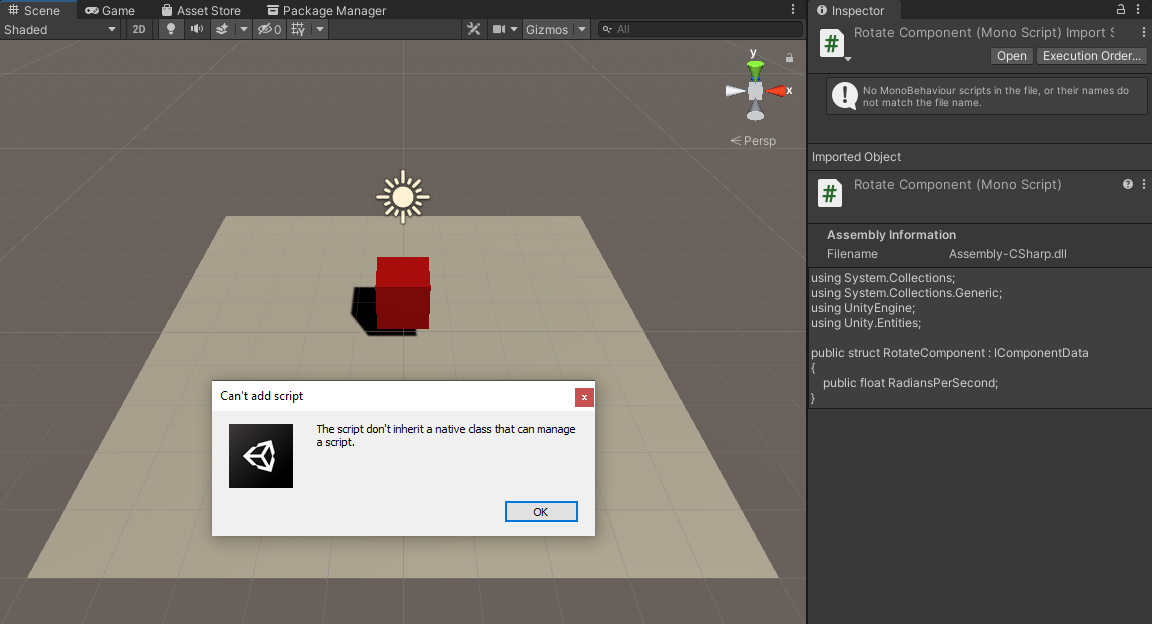
\includegraphics[width=0.95\columnwidth]{gfx/imgs/chapter2/NonAuthoringComponentExample.png}
    \caption{Componente senza tag \UseVerb{[GenerateAuthoringComponent]Term}.}
    \label{fig:non-authoring-example}
\end{figure}

\begin{figure}[!ht]
    \centering
    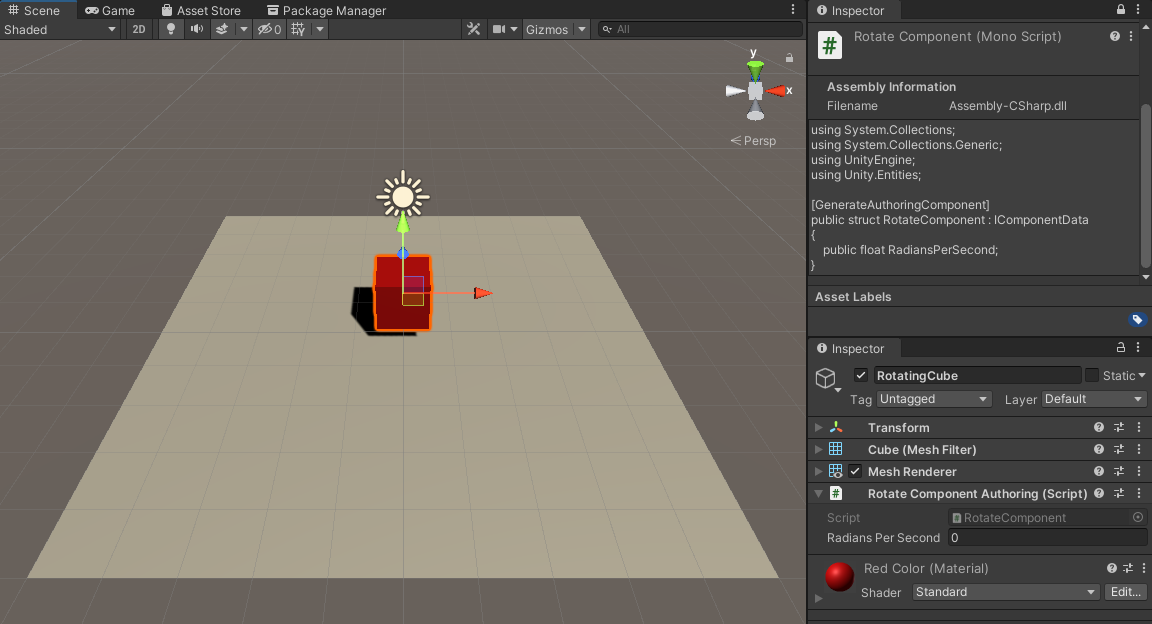
\includegraphics[width=0.95\columnwidth]{gfx/imgs/chapter2/AuthoringComponentExample.png}
    \caption{Componente con tag \UseVerb{[GenerateAuthoringComponent]Term}.}
    \label{fig:authoring-example}
\end{figure}

\subsubsection{Sistemi di conversione}
I sistemi di conversione ereditano dalla classe \verb|GameObjectConversionSystem| e permettono di convertire GameObject ed asset in entità. Di default aggiornano nel gruppo \verb|GameObjectConversionGroup| e una delle differenze più consistenti rispetto ai sistemi normali di ECS è che quelli di conversione non si trovano in un World singolo ma stanno a cavallo di due: leggono dal Conversion World (quello in cui si trovano gli authoring data) e scrivono nel Destination World (in cui si trovano le entità).

Durante la conversione, per ogni GameObject processato viene creata l'entità corrispondente.
Inoltre, i sistemi di conversione eseguono sul main thread senza burst, infatti il costrutto \verb|Entities.ForEach| non richiede la chiamata a metodi \verb|Run()| o \verb|Schedule()| quando viene utilizzato all'interno di questi~\cite{doc:unity-entities-api}.

\subsubsection{Interfaccia IConvertGameObjectToEntity}
Un metodo più semplice rispetto alla creazione di un sistema di conversione consiste nell'implementare l'interfaccia \verb|IConvertGameObjectToEntity| nella classe del \verb|MonoBehaviour| contenente il componente. Questa interfaccia fornisce un metodo con il quale possiamo realizzare una conversione personalizzata. Praticamente permette di personalizzare ciò che l'attributo \verb|[GenerateAuthoringComponent]| realizza in modo trasparente.

Durante l'aggiornamento del gruppo \verb|GameObjectConversionGroup|, viene chiamato il metodo \verb|Convert()| di tutti i componenti che implementano questa interfaccia ~\cite{doc:unity-entities-manual}.

\SaveVerb{IConvertGameObjectToEntityTerm}|IConvertGameObjectToEntity|

\begin{lstlisting}[caption={Esempio di conversione personalizzata tramite l'utilizzo dell'interfaccia \UseVerb{IConvertGameObjectToEntityTerm}~\cite{youtube:conversione-dati-scene-dots}.}, label={lst:convert-example}, language={[Sharp]C}]
public struct RotateComponent : IComponentData
{
	public float RadiansPerSecond;
}

public class RotateComponentAuthoring : MonoBehaviour, IConvertGameObjectToEntity
{
	public float DegreesPerSecond

	public void Convert(Entity entity, EntityManager dstManager, GameObjectConversionSystem conversionSystem)
	{
		dstManager.AddComponentData(entity, 
		new Rotate { RadiansPerSecond = math.radians(DegreesPerSecond) });
	}
}
\end{lstlisting}

%subsubsection{Prefabs}

%\subsubsection{Conversione in LiveLink} % forse non serve, nel prototipo non è stato utilizzato (volendo c'è scritto qualcosa di veloce nella descrizione del package Entities)
% IJobEntityBatch (API) c'è scritta molta roba utile